\todo[inline, size=normalsize]{Falar dos problemas multifásicos rapidamente, explicando bem por cima o que é um problema multifásico.}

\todo[inline, color=pink, size=normalsize]{Descrição geral do problema}

O estudo de caso em análise consiste na determinação da trajetória a ser percorrida por um foguete Delta III para que o mesmo atinja uma determinada órbita, de forma que seja maximizada a quantidade de combustível restante ao fim do voo. Vale ressaltar que quanto menos combustível for gasto para fazer com que o foguete chegue até a órbita alvo, mais propelente poderá ser empregado na rejeição de perturbações \cite{benson_gauss_2005}.

O Delta III possui dois estágio e nove propulsores de propelente sólido (PPS). A trajetória percorrida pelo mesmo pode ser divida em quatro fases. Na primeira fase, seis dos nove PPS queimam ao mesmo tempo que o propulsor do primeiro estágio, sendo os PPS descartados assim que o combustível neles armazenado tenha se esgotado. Se inicia então a segunda fase, na qual os três PPS restantes queimam ao mesmo tempo que o propulsor do primeiro estágio. Mais uma vez, os PPS são descartados assim que o combustível neles armazenado se esgota. Tem início a terceira fase, na qual ocorre apenas a queima do propulsor do primeiro estágio. Uma vez que o propelente armazenado nesse estágio chega ao fim, descarta-se o mesmo e da-se início à quarta e última fase, na qual queima apenas o propulsor do segundo estágio. Ao fim da quarta fase, o Delta III deve ter alcançado a órbita alvo, e a carga útil nele armazenada deve ser liberada. 

A resolução do estudo de caso em análise é baseada na formulação de um PCO com múltiplas fases. O processo de transcrição de PCOs desse tipo é semelhante ao de PCOs monofásicos, sendo a função objetivo determinada a partir da somatória das funções objetivo associadas a cada fase, e tratando-se os estados e controles referentes a cada fase como variáveis de projeto distintas. Além disso, pode ser necessário que novas restrições sejam estabelecidas para garantir que os estados de uma fase se conectem aos da seguinte sem que haja descontinuidades \cite{becerra_psopt_2019}. 

As variáveis empregadas na formulação do estudo de caso em análise são apresentadas na Figura \ref{fig:foguete:foguete},

\noindent	
\begin{minipage}{\textwidth}
	\vspace{\onelineskip}
	\centering
	\includegraphics[width=0.75\linewidth]{draw/resultados/pdf/foguete}
	\captionof{figure}[Representação esquemática do problema do lançamento de um foguete]{Representação esquemática do problema do lançamento de um foguete.}
	\label{fig:foguete:foguete}
	\vspace{\onelineskip}
\end{minipage}
%
sendo $ T $ a força de empuxo gerada pela queima dos propulsores, $ \mathbf{u}(t) $ o vetor unitário que indica a direção de $ T $, $ \mathbf{r}(t) $ a posição do foguete em relação ao centro da Terra, e $ \mathbf{v}(t) $ a velocidade associada ao mesmo. A massa, a área de referência, e o coeficiente de arrasto do foguete são denotados, respectivamente, por $ m $, $ A_{ref} $ e $ c_d $. O impulso específico associado aos propulsores e o arrasto aerodinâmica são denotado, respectivamente, por $ I $ e $ \mathbf{D} $. O raio e taxa de rotação da Terra, assim como o parâmetro gravitacional associado à mesma, são denotados por $ R_e $, $ \omega_e $ e $ \mu $, respectivamente. Por fim, $ g_0 $ e $ \rho_0 $ são a aceleração da gravidade e a densidade do ar atmosférico no nível do mar. 

Vale ressaltar que as equações de movimento do Delta III são aqui formuladas com base no sistema de coordenadas inercial centrado na Terra (ECI ou \textit{Earth Centered Inertial}), Figura \ref{fig:foguete:eci}. Nesse caso, o plano $ xy $ coincide com o plano equatorial, enquanto o eixo $ z $ aponta na direção do polo norte. Esse sistema de coordenadas é fixo com relação às estrelas e não acompanha o movimento de rotação da Terra.  

\noindent	
\begin{minipage}{\textwidth}
	\vspace{\onelineskip}
	\centering
	\includegraphics[width=0.65\linewidth]{draw/resultados/pdf/coordenadasECI}
	\captionof{figure}[Sistema de coordenadas inercial centrado na Terra]{Sistema de coordenadas inercial centrado na Terra.}
	\label{fig:foguete:eci}
	\vspace{\onelineskip}
\end{minipage}

\todo[inline, color=pink, size=normalsize]{Apresentação das equações dinâmicas - Equações, Estados, Controles e Valor inicial dos estados}

A dinâmica do foguete Delta III é descrita pelo sistema de equações \eqref{eq:foguete:dinamica},
%
\begin{equation}
	\label{eq:foguete:dinamica}
	\begin{gathered}
		\dot{\mathbf{r}}(t) = \mathbf{v}(t) \\
		\dot{\mathbf{v}}(t) = -\frac{\mu}{|\mathbf{r}(t)|^3} \mathbf{r}(t) + \frac{T(t)}{m(t)} \mathbf{u}(t) + \frac{\mathbf{D}(t)}{m(t)} \\
		\dot{m}(t) = dm(t)
	\end{gathered}
\end{equation}
%
sendo
%
\begin{equation}
	\begin{gathered}
		\mathbf{r}(t) = \begin{bmatrix} r_x(t) & r_y(t) & r_z(t) \end{bmatrix}^T \\
		\mathbf{v}(t) = \begin{bmatrix} v_x(t) & v_y(t) & v_z(t) \end{bmatrix}^T \\
		\mathbf{D}(t) = \begin{bmatrix} D_x(t) & D_y(t) & D_z(t) \end{bmatrix}^T \\
		\mathbf{u}(t) = \begin{bmatrix} u_x(t) & u_y(t) & u_z(t) \end{bmatrix}^T 
	\end{gathered}
\end{equation}

O arrasto aerodinâmico $ \mathbf{D}(t) $ deve ser computado segundo \eqref{eq:foguete:arrasto}, 
%
\begin{equation}
	\label{eq:foguete:arrasto}
	\mathbf{D}(t) = -\frac{1}{2} \, c_d \, A_{ref} \, \rho(t) \, |\mathbf{v_{ref}}(t)| \, \mathbf{v_{ref}}(t)
\end{equation}
%
em que $ \mathbf{v_{ref}}(t) $ é a velocidade do foguete em relação à atmosfera. Considerando-se que o ar atmosférico se move juntamente com a Terra, e que $ {\bm \omega} = \begin{bmatrix} 0 & 0 & \omega_e \end{bmatrix} $ tem-se
%
\begin{equation}
	\mathbf{v_{ref}}(t) = \mathbf{v}(t) + {\bm \omega} \times \mathbf{r}(t)
\end{equation}

Além disso, a densidade $ \rho(t) $ do ar atmosférico a uma dada altitude $ h(t) $, sendo
%
\begin{equation}
	\label{eq:foguete:altitude}
	h(t) = |\mathbf{r}(t)| - R_e
\end{equation}
%
deve ser computada segundo \eqref{eq:foguete:densidadeAr},
%
\begin{equation}
	\label{eq:foguete:densidadeAr}
	\rho(t) = \rho_0 \, e^{-h(t)/h_0}
\end{equation} 
%
sendo $ h_0 $ um fator de ponderação da altitude. 

As equações de movimento  \eqref{eq:foguete:dinamica} podem ser empregadas em qualquer uma das fases do voo, devendo-se levar em conta o empuxo $ T(t) $ e a taxa de variação de massa $ dm(t) $ associados a cada fase. Em \eqref{eq:foguete:empuxos} e \eqref{eq:foguete:massas} são introduzidos os $ T(t) $ e $ dm(t) $ atribuídos a cada fase, sendo $ T_{sb} $, $ T_{s1} $ e $ T_{s2} $ os empuxos gerados por um PPS e pelos propulsores do primeiro e segundo estágio respectivamente \cite{becerra_psopt_2019}. De forma análoga, as taxas de variação de massa referentes a cada um dos propulsores do Delta III são denotadas por $ dm_{sb} $, $ dm_{s1} $ e $ dm_{s2} $. A cada um dos $ T(t) $ e $ dm(t) $ é atribuído um sobrescrito que indica o número da fase. 
%
\begin{gather}
	\label{eq:foguete:empuxos}
	\begin{gathered}
		T^{(1)} = 6 \, T_{sb} + T_{s1} \\
		T^{(2)} = 3 \, T_{sb} + T_{s1} \\
		T^{(3)} = T_{s1} \\
		T^{(4)} = T_{s2}
	\end{gathered} \\
	\label{eq:foguete:massas}
	\begin{gathered}
		dm^{(1)} = -6 \, dm_{sb} - dm_{s1} \\
		dm^{(2)} = -3 \, dm_{sb} - dm_{s1} \\
		dm^{(3)} = - dm_{s1} \\
		dm^{(4)} = - dm_{s2} \\
	\end{gathered} 
\end{gather}
%
A determinação de $ dm_{sb} $, $ dm_{s1} $ e $ dm_{s2} $ se dá pelo emprego de  \eqref{eq:foguete:determinacaoDm},
%
\begin{equation}
	\label{eq:foguete:determinacaoDm}
	\begin{gathered}
		dm_{sb} = \frac{T_{sb}}{g_0 \, I_{sb}} \\
		dm_{s1} = \frac{T_{s1}}{g_0 \, I_{s1}} \\
		dm_{s2} = \frac{T_{s2}}{g_0 \, I_{s2}}
	\end{gathered}
\end{equation}
% 
sendo $ I_{sb} $, $ I_{s1} $, e $ I_{s2} $ definidos a partir da massa de combustível e do tempo de queima de cada propulsor. No caso dos PPS tem-se
%
\begin{equation}
I_{sb} = \frac{1}{g_0} \, \frac{T_{sb}}{m_{sb}/t_{sb}}
\end{equation}
%
sendo $ m_{sb} $ a massa do propelente armazenado em cada um dos propulsores, e $ t_{sb} $ o tempo de queima associado aos mesmos. De forma análoga, considerando-se $ m_{s1} $, $ m_{s2} $, $ t_{s1} $ e $ t_{s1} $, como sendo, respectivamente, as massas do combustível armazenado no primeiro e segundo estágios, e o tempo de queima associado aos mesmos, obtém-se $ I_{s1} $ e $ I_{s2} $ \cite{becerra_psopt_2019}.

Considera-se que $ \mathbf{x}(t) = \begin{bmatrix} r_x(t) & r_y(t) & r_z(t) & v_x(t) & v_y(t) & v_z(t) & m(t) \end{bmatrix}^T $ e $ \mathbf{u}(t) = \begin{bmatrix} u_x(t) & u_y(t) & u_z(t) \end{bmatrix}^T $ são, respectivamente, os estados e controles associados à dinâmica do Delta III. As condições iniciais atribuídas a $ \mathbf{x}(t) $ são introduzidas em \eqref{eq:foguete:inicial}.
%
\begin{gather}
	\label{eq:foguete:inicial}
		\begin{gathered}
			\mathbf{r}(0) = \mathbf{r_0} \\
			\mathbf{v}(0) = \mathbf{v_0} \\
			m(0) = m_0
		\end{gathered}	
\end{gather}

Considerando como local de lançamento o Cabo Canaveral, na Flórida, que possui latitude $ l_{cc} $, determina-se $ \mathbf{r_0} $ da seguinte forma \cite{becerra_psopt_2019}:
%
\begin{equation}
	\label{eq:foguete:r0Calculo}
	\mathbf{r}_0 = 
	\begin{bmatrix}
		r_{0x} \\
		r_{0y} \\
		r_{0z} 
	\end{bmatrix} = 
	\begin{bmatrix}
		R_e \; cos \, l_{cc} \\
		0 \text{ m}\\
		R_e \; sen \, l_{cc}
	\end{bmatrix} 
\end{equation}

De fato, qualquer ponto $ P $ na superfície da Terra pode ser posicionado determinando-se a latitude, a longitude e a altitude associadas ao mesmo, Figura \ref{fig:foguete:latitudeLongitude} \cite{britannica_escola_latitude_2020}.

\noindent	
\begin{minipage}{\textwidth}
	\vspace{\onelineskip}
	\centering
	\includegraphics[width=0.65\linewidth]{draw/resultados/pdf/coordenadasLaLo}
	\captionof{figure}[Posicionamento de um ponto qualquer na superfície terrestre utilizando-se a latitude e a longitude]{Posicionamento de um ponto qualquer $ P $ na superfície terrestre por meio da determinação da latitude e da longitude associadas ao mesmo. Considerando-se que o ponto $ P $ se encontra na superfície da Terra, a altitude associada ao mesmo é nula.}
	\label{fig:foguete:latitudeLongitude}
	\vspace{\onelineskip}
\end{minipage}

A velocidade $ \mathbf{v_0} $ por sua vez é determinada com base na relação $ \mathbf{v}_0 = {\bm \omega} \times \mathbf{r}_0 $ \cite{becerra_psopt_2019}. Assim sendo, 
%
\begin{equation}
	\mathbf{v}_0 = 
	\begin{bmatrix}
		v_{0x} \\
		v_{0y} \\
		v_{0z}
	\end{bmatrix} = 
	\begin{bmatrix}
		- r_{0y} \, w_e \\
		r_{0x} \, w_e \\
		0 \text{ m/s}
	\end{bmatrix}
\end{equation}

Por fim, considerando-se $ M_{sb} $, $ M_{s1} $, $ M_{s2} $, e $ m_{pl} $ as massas de um dos PPS, do propulsor do primeiro estágio, do propulsor do segundo estágio, e da carga útil, respectivamente, determina-se a massa inicial $ m_0 $ do Delta III \cite{becerra_psopt_2019}
%
\begin{equation}
	m_0 = 9 \, M_{sb} + M_{s1} + M_{s2} + m_{pl}
\end{equation}

\todo[inline, color=pink, size=normalsize]{Apresentação da função objetivo}

Uma vez que pretende-se maximizar o combustível restante no segundo estágio quando o foguete alcança a órbita alvo, considera-se a minimização da função objetivo introduzida em \eqref{eq:foguete:objetivo}
%
\begin{equation}
	\label{eq:foguete:objetivo}
	J = -m(t_f^{(4)})
\end{equation}
%
sendo $ t_f^{(4)} $ o tempo final da última fase da trajetória percorrida pelo Delta III. 

\todo[inline, color=pink, size=normalsize]{Apresentação das restrições - Restrições laterais}

As restrições associadas a $ \mathbf{r}(t) $ e $ \mathbf{v}(t) $ são introduzidas em \eqref{eq:foguete:laterais} \cite{becerra_psopt_2019}. 
%
\begin{equation}
	\label{eq:foguete:laterais}
	\begin{gathered}
		0 \leq r_x(t) \leq 2 \, R_e \\
		0 \leq r_y(t) \leq 2 \, R_e \\
		0 \leq r_z(t) \leq 2 \, R_e \\
		-20000 \text{ m/s} \leq v_x(t) \leq 20000 \text{ m/s}\\
		-20000 \text{ m/s} \leq v_y(t) \leq 20000 \text{ m/s}\\
		-20000 \text{ m/s} \leq v_z(t) \leq 20000 \text{ m/s}
	\end{gathered}
\end{equation}

Para que as restrições referentes a $ m(t) $ possam ser determinadas, é necessário primeiramente definir qual é a massa total do foguete no início e no fim de cada uma das fases. Considerando-se que o propelente de todos os propulsores queima de forma contínua tem-se
%
\begin{equation}
\begin{gathered}
m^{(1)} \left( t_0^{(1)} \right) = m_0 \\
m^{(1)} \left( t_f^{(1)} \right) = m^{(1)} \left( t_0^{(1)} \right) - \left( 6 \, \frac{m_{sb}}{t_{sb}} + \frac{m_{s1}}{t_{s1}} \right) t_f^{(1)} \\
m^{(2)} \left( t_0^{(2)} \right) = m^{(1)} \left( t_f^{(1)} \right) - 6 \, (M_{sb} - m_{sb}) \\
m^{(2)} \left( t_f^{(2)} \right) = m^{(2)} \left( t_0^{(2)} \right) - \left( 3 \, \frac{m_{sb}}{t_{sb}} + \frac{m_{s1}}{t_{s1}} \right) \left( t_f^{(2)} - t_f^{(1)} \right) \\
m^{(3)} \left( t_0^{(3)} \right) = m^{(2)} \left( t_f^{(2)} \right) - 3 \, (M_{sb} - m_{sb}) \\
m^{(3)} \left( t_f^{(3)} \right) = m^{(3)} \left( t_0^{(3)} \right) - \left( \frac{m_{s1}}{t_{s1}} \right) \left( t_f^{(3)} - t_f^{(2)} \right) \\
m^{(4)} \left( t_0^{(4)} \right) = m^{(3)} \left( t_f^{(3)} \right) - ( M_{s1} - m_{s1} ) \\
\end{gathered}
\end{equation}
%
sendo $ t_0^{(i)} $ o tempo inicial da $ i $-ésima fase. Vale ressaltar que $ m^{(4)} \left( t_0^{(4)} \right) $ deve ser determinado por meio da resolução do estudo de caso em análise. 

Assim sendo, as restrições associadas a $ m(t) $ são introduzidas em \eqref{eq:foguete:lateraisMassa} \cite{becerra_psopt_2019}.
%
\begin{equation}
	\label{eq:foguete:lateraisMassa}
	\begin{gathered}
		m^{(1)} \left( t_0^{(1)} \right) \leq m^{(1)}(t) \leq m^{(1)} \left( t_f^{(1)} \right) \\
		m^{(2)} \left( t_0^{(2)} \right) \leq m^{(2)}(t) \leq m^{(2)} \left( t_f^{(2)} \right) \\
		m^{(3)} \left( t_0^{(3)} \right) \leq m^{(3)}(t) \leq m^{(3)} \left( t_f^{(3)} \right) \\
		m^{(4)} \left( t_0^{(4)} \right) \leq m^{(4)}(t) \leq m^{(4)} \left( t_f^{(4)} \right) \\
	\end{gathered}
\end{equation}

Os tempos inicial e final de cada fase estão diretamente relacionados ao tempo de queima associado a cada propulsor, 
%
\begin{equation}
	\begin{gathered}
		t_0^{(1)} = 0 \\
		t_f^{(1)} = t_0^{(2)} = t_{sb} \\
		t_f^{(2)} = t_0^{(3)} = 2 \, t_{sb} \\
		t_f^{(3)} = t_0^{(4)} = t_{s1} 
	\end{gathered}
\end{equation}

Vale ressaltar que o tempo final $ t_f^{(4)} $ deve ser determinado por meio da resolução do estudo de caso em análise.

\todo[inline, color=pink, size=normalsize]{Apresentação das restrições - Restrições terminais}

A órbita alvo é especificada por meio dos elementos orbitais
%
\begin{equation}
	\label{eq:foguete:orbitaTerminal}
	\begin{gathered}
		a(t_f^{(4)}) = a_f \\
		e(t_f^{(4)}) = e_f \\
		i(t_f^{(4)}) = i_f \\
		\Omega(t_f^{(4)}) = \Omega_f \\
		\omega(t_f^{(4)}) = \omega_f 
	\end{gathered}
\end{equation}
%
sendo $ a(t) $ o semi-eixo maior, $ e(t) $ a excentricidade, $ i(t) $ a inclinação, $ \Omega(t) $ a longitude do nó ascendente, e $ \omega(t) $ o argumento do periapsis. Essas grandezas podem ser determinadas a partir de $ \mathbf{r}(t) $ e $ \mathbf{v}(t) $ com base nas equações apresentadas ao fim dessa seção. Na Figura \ref{fig:foguete:orbitais} são representadas alguns dos elementos orbitais. Uma vez que não há uma restrição terminal atribuída à anomalia verdadeira $ \nu(t) $, não há uma posição específica na órbita que o foguete deve atingir. As coordenadas $ a(t) $ e $ e(t) $ não foram representadas na Figura \ref{fig:foguete:orbitais} mas denotam a excentricidade e o semi-eixo maior da elipse associada à órbita na qual o foguete se encontra. 

\noindent	
\begin{minipage}{\textwidth}
	\vspace{\onelineskip}
	\centering
	\includegraphics[width=0.7\linewidth]{draw/resultados/pdf/coordenadasOrbitais}
	\captionof{figure}[Representação dos elementos orbitais]{Representação dos elementos orbitais.}
	\label{fig:foguete:orbitais}
	\vspace{\onelineskip}
\end{minipage}


\todo[inline, color=pink, size=normalsize]{Apresentação das restrições - Restrições de caminho}

Uma vez que o vetor $ \mathbf{u}(t) $ precisa ser unitário, deve-se impor que 
%
\begin{equation}
	|\mathbf{u}(t)| = 1	
\end{equation}

Além disso, visando garantir que as trajetórias obtidas não transpassem a Terra, é necessário que o foguete se mantenha sempre acima do solo, de forma que
%
\begin{equation}
	|\mathbf{r}(t)| \geq R_e	
\end{equation}

\todo[inline, color=pink, size=normalsize]{Apresentação das restrições - Restrições entre fases}

Por fim, é necessário garantir que as posições e velocidades do foguete se mantenham contínuas ao longo de toda a trajetória. Para tanto, devem ser respeitadas as seguintes restrições,
%
\begin{gather}
\label{eq:foguete:rContinua}
\begin{gathered}
\mathbf{r}^{(2)} \left( t_0^{(2)} \right) = \mathbf{r}^{(1)} \left( t_f^{(1)} \right) \\
\mathbf{r}^{(3)} \left( t_0^{(3)} \right) = \mathbf{r}^{(2)} \left( t_f^{(2)} \right) \\
\mathbf{r}^{(4)} \left( t_0^{(4)} \right) = \mathbf{r}^{(3)} \left( t_f^{(3)} \right) 
\end{gathered} \\
\label{eq:foguete:vContinua}
\begin{gathered}
\mathbf{v}^{(2)} \left( t_0^{(2)} \right) = \mathbf{v}^{(1)} \left( t_f^{(1)} \right) \\
\mathbf{v}^{(3)} \left( t_0^{(3)} \right) = \mathbf{v}^{(2)} \left( t_f^{(2)} \right) \\
\mathbf{v}^{(4)} \left( t_0^{(4)} \right) = \mathbf{v}^{(3)} \left( t_f^{(3)} \right) 
\end{gathered}
\end{gather}
%
ao passo que, para que as variações de massa ocasionadas pelo descarte dos PPS e do primeiro estágio sejam consideradas, tem-se que
%
\begin{equation}
	\begin{gathered}
		m^{(2)} \left( t_0^{(2)} \right)  = m^{(1)} \left( t_f^{(1)} \right) - \Delta m^{(1)} \\
		m^{(3)} \left( t_0^{(3)} \right)  = m^{(2)} \left( t_f^{(2)} \right) - \Delta m^{(2)} \\
		m^{(4)} \left( t_0^{(4)} \right)  = m^{(3)} \left( t_f^{(3)} \right) - \Delta m^{(3)} 			
	\end{gathered}
\end{equation}
%
sendo $ \Delta m^{(1)} $, $ \Delta m^{(2)} $ e $ \Delta m^{(3)} $ a massa descartada em cada um das fases
%
\begin{equation}
	\begin{gathered}
		\Delta m^{(1)} = 6 \, (M_{sb} - m_{sb}) \\
		\Delta m^{(2)} = 3 \, (M_{sb} - m_{sb}) \\
		\Delta m^{(3)} = M_{s1} - m_{s1}
	\end{gathered}
\end{equation}

\todo[inline, color=pink, size=normalsize]{Considerações específicas de cada problema - palpites iniciais associados a cada fase}

Os palpites inicias associados a $ \mathbf{r}(t) $ são apresentados em \eqref{eq:foguete:rIniciais}
%
\begin{equation}
	\label{eq:foguete:rIniciais}
	\begin{gathered}
		\mathbf{r}_p^{(1)}(t) = \mathbf{r_0} \\
		\mathbf{r}_p^{(2)}(t) = \mathbf{r_0} \\
		\mathbf{r}_p^{(3)}(t) = \mathbf{r_f} \\
		\mathbf{r}_p^{(4)}(t) = \mathbf{r_f} 
	\end{gathered}
\end{equation}
%
enquanto os associados a $ \mathbf{v}(t) $ são introduzidos em \eqref{eq:foguete:vIniciais}
%
\begin{equation}
	\label{eq:foguete:vIniciais}
	\begin{gathered}
		\mathbf{v}_p^{(1)}(t) = \mathbf{v_0} \\
		\mathbf{v}_p^{(2)}(t) = \mathbf{v_0} \\
		\mathbf{v}_p^{(3)}(t) = \mathbf{v_f} \\
		\mathbf{v}_p^{(4)}(t) = \mathbf{v_f} 
	\end{gathered}
\end{equation}
%
sendo $ \mathbf{r_f} = \begin{bmatrix} r_{fx} & r_{fy} & r_{fz} \end{bmatrix} $ e $ \mathbf{v_f} = \begin{bmatrix} v_{fx} & v_{fy} & v_{fz} \end{bmatrix} $ quaisquer posições e velocidades que atendam às condições terminais. Uma vez que o Delta III deve alcançar uma órbita pré-determinada, e não uma posição específica, há várias combinações de $ \mathbf{r}(t_f) $ e $ \mathbf{v}(t_f) $ que satisfazem \eqref{eq:foguete:orbitaTerminal}. A combinação aqui adotada é obtida considerando-se $ \nu = 0 $ \cite{becerra_psopt_2019}. 

Os palpites iniciais atribuídos a $ \mathbf{u}(t) $ são introduzidos em \eqref{eq:foguete:uIniciais}
%
\begin{equation}
	\label{eq:foguete:uIniciais}
	\begin{gathered}
		\mathbf{u}_p^{(1)}(t) = \mathbf{u_0} \\
		\mathbf{u}_p^{(2)}(t) = \mathbf{u_0} \\
		\mathbf{u}_p^{(3)}(t) = \mathbf{u_f} \\
		\mathbf{u}_p^{(4)}(t) = \mathbf{u_f} 
	\end{gathered}
\end{equation}
%
sendo $ \mathbf{u_0} = \begin{bmatrix} 1 & 0 & 0\end{bmatrix} $ e $ \mathbf{u_f} = \begin{bmatrix} 0 & 0 & 1\end{bmatrix} $ \cite{becerra_psopt_2019}.

Por fim, os palpites iniciais associados à $ m(t) $ são introduzidos em \eqref{eq:foguete:massaPalpites}.
%
\begin{equation}
	\label{eq:foguete:massaPalpites}
	\begin{gathered}
		m_p^{(1)}(t) = m^{(1)} \left( t_0^{(1)} \right) \\
		m_p^{(2)}(t) = m^{(2)} \left( t_0^{(2)} \right) \\
		m_p^{(3)}(t) = m^{(3)} \left( t_0^{(3)} \right) \\
		m_p^{(4)}(t) = m^{(4)} \left( t_0^{(4)} \right) 
	\end{gathered}
\end{equation}

\todo[inline, color=pink, size=normalsize]{Tabela das constantes do problema}

A seguir estão listados os parâmetros utilizados na formulação do estudo de caso em análise e os valores a eles atribuídos:
%
\begin{itemize}
	\item Raio da Terra: $ R_e = 6378145 $ \text{m}
	\item Taxa de rotação da Terra em torno do eixo $ z $: $ w_e = 7,29211585 \times 10^{-5} $ \text{ rad/s}
	\item Aceleração da gravidade ao nível do mar: $ g_0 = 9,80665 $ \text{ m/s$^2$}
	\item Densidade do ar atmosférico ao nível do mar: $ \rho_0 = 1,225 $ \text{ kg/m$^3$}
	\item Parâmetro gravitacional: $ \mu = 3,986012 \times 10^{14} $ \text{ m$^3$/s$^2$}
	\item Coeficiente de arrasto aerodinâmico associado ao Delta III: $ c_d = 0,5 $ 
	\item Área de referência do Delta III: $ A_{ref} = 4 \pi $ \text{ m$^2$}
	\item Fator de ponderação da altitude: $ h_0 = 7200 $ \text{ m}
	\item Massa da carga útil: $ m_{pl} = 4164$ \text{ kg}
	\item Latitude do Cabo Canaveral (local de lançamento):  $l_{cc} = 28,5 \degree $
	\item Empuxo de um PPS: $ T_{sb} = 628500 $ \text{ N}
	\item Empuxo do propulsor do primeiro estágio: $ T_{s1} = 1083100 $ \text{ N}
	\item Empuxo do propulsor do segundo estágio: $ T_{s2} = 110094 $ \text{ N}
	\item Tempo de queima de um PPS: $ t_{sb} = 75,2 $ \text{ s}
	\item Tempo de queima do propulsor do primeiro estágio: $ t_{s1} = 261 $ \text{ s}
	\item Tempo de queima do propulsor do segundo estágio: $ t_{s2} = 700 $ \text{ s}
	\item Massa total de um PPS: $ M_{sb} = 19290 $ \text{ kg}
	\item Massa total do primeiro estágio: $ M_{s1} = 104380 $ \text{ kg}
	\item Massa total do segundo estágio: $ M_{s2} = 19300 $ \text{ kg}
	\item Massa do combustível armazenado em um PPS: $ m_{sb} = 17010 $ \text{ kg}
	\item Massa do combustível armazenado no primeiro estágio: $ m_{s1} = 95550 $ \text{ kg}
	\item Massa do combustível armazenado no segundo estágio: $ m_{s2} = 16820 $ \text{ kg}
	\item Componente em $ x $ da posição inicial do Delta III: $ r_{0x} = 5605222 $ \text{ m}
	\item Componente em $ y $ da posição inicial do Delta III: $ r_{0y} = 0 $ \text{ m}
	\item Componente em $ z $ da posição inicial do Delta III: $ r_{0y} = 3043387 $ \text{ m}
	\item Componente em $ x $ da velocidade inicial do Delta III: $ v_{0x} = 0 $ \text{ m/s}
	\item Componente em $ y $ da velocidade inicial do Delta III: $ v_{0y} = 409 $ \text{ m/s}
	\item Componente em $ z $ da velocidade inicial do Delta III: $ v_{0z} = 0 $ \text{ m/s}
	\item Componente em $ x $ de uma das possíveis posições finais do Delta III: $ r_{fx} = 4397287 $ \text{ m}
	\item Componente em $ y $ de uma das possíveis posições finais do Delta III: $ r_{fy} = 4243769 $ \text{ m}
	\item Componente em $ z $ de uma das possíveis posições finais do Delta III: $ r_{fz} = 2379474 $ \text{ m}
	\item Componente em $ x $ de uma das possíveis velocidades finais do Delta III: $ v_{fx} = -5826 $ \text{ m/s}
	\item Componente em $ y $ de uma das possíveis velocidades finais do Delta III: $ v_{fy} = 7819 $ \text{ m/s}
	\item Componente em $ z $ de uma das possíveis velocidades finais do Delta III: $ v_{fz} = -3178$ \text{ m/s}
	\item Massa total do Delta III no início da 1ª fase: $ m^{(1)} \left( t_0^{(1)} \right) = 301454$ \text{ kg}
	\item Massa total do Delta III ao fim da 1ª fase: $ m^{(1)} \left( t_f^{(1)} \right) = 171864$ \text{ kg}
	\item Massa total do Delta III no início da 2ª fase: $ m^{(2)} \left( t_0^{(2)} \right) = 158184$ \text{ kg}
	\item Massa total do Delta III ao fim da 2ª fase: $ m^{(2)} \left( t_f^{(2)} \right) = 79624$ \text{ kg}
	\item Massa total do Delta III no início da 3ª fase: $ m^{(3)} \left( t_0^{(3)} \right) = 72784$ \text{ kg}
	\item Massa total do Delta III ao fim da 3ª fase: $ m^{(3)} \left( t_f^{(3)} \right) = 32294$ \text{ kg}
	\item Massa total do Delta III no início da 4ª fase: $ m^{(4)} \left( t_0^{(4)} \right) = 23464$ \text{ kg}
	\item Semi-eixo maior associado à orbita final do Delta III: $ a_f = 24361140 $ \text{m}
	\item Excentricidade associada à orbita final do Delta III: $ e_f = 0,7308 $
	\item Inclinação associada à orbita final do Delta III: $ i_f = 28,5 \degree$ 
	\item Longitude do nó ascendente associada à orbita final do Delta III: $ \Omega_f = 269,8 \degree$
	\item Argumento do periapsis associado à orbita final do Delta III: $ \omega_f = 130,5 \degree$ 
\end{itemize}

\todo[inline, color=pink, size=normalsize]{Considerações específicas de cada problema - hipóteses simplificadoras}

Vale ressaltar, por fim, algumas hipóteses simplificadoras que foram adotadas na formulação do estudo de caso em análise. Primeiramente, é atribuído a cada motor o empuxo produzido no vácuo, sem que seja considerada qualquer influência da pressão atmosférica. Além disso, supõe-se que $ A_{ref} $ e $ c_d $ não dependem do ângulo de ataque do foguete ou do número de Mach associado ao mesmo, e que o arrasto atua sempre no sentido oposto à velocidade, sem que haja quaisquer forças de sustentação. Por fim, para que seja possível determinar $ h(t) $ e $ \mathbf{r_0} $ empregando-se, respectivamente, \eqref{eq:foguete:altitude} e \eqref{eq:foguete:rIniciais}, e para que o modelo gravitacional de massa pontual seja satisfeito, assume-se que a Terra é esférica. 

\todo[inline, color=pink, size=normalsize]{Apresentação da análise de sensibilidade $ J \times N $ para definição de $ N_m $ }

São apresentados na Figura \ref{fig:foguete:sensibilidade:J} os resultados obtidos a partir da análise de sensibilidade com base na qual foi determinado o número mínimo de nós de colocação $ N_m $, que se encontra indicado em cada gráfico. A coleta dos dados em questão foi realizada atribuindo-se a $ N $ trinta valores distintos, linearmente espaçados entre 5 e 34. Avaliando-se tais resultados, é possível verificar a influência que o número de nós de colocação $ N $ tem sobre o valor ótimo da função objetivo $ J^* $. 

Vale ressaltar que são apresentados nessa seção apenas os resultados obtidos por meio do $ PSOPT $, uma vez que o $ COPILOTS $ não possui suporte para problemas com múltiplas fases, e que não foi possível resolver o estudo de caso em análise por meio do $ FALCON $. Apesar desse último pacote ser capaz de resolver problemas com múltiplas fases, não foi verificada a convergência do processo de otimização quando o mesmo foi empregado.

\noindent	
\begin{minipage}{\textwidth}
	\vspace{\onelineskip}
	\centering
	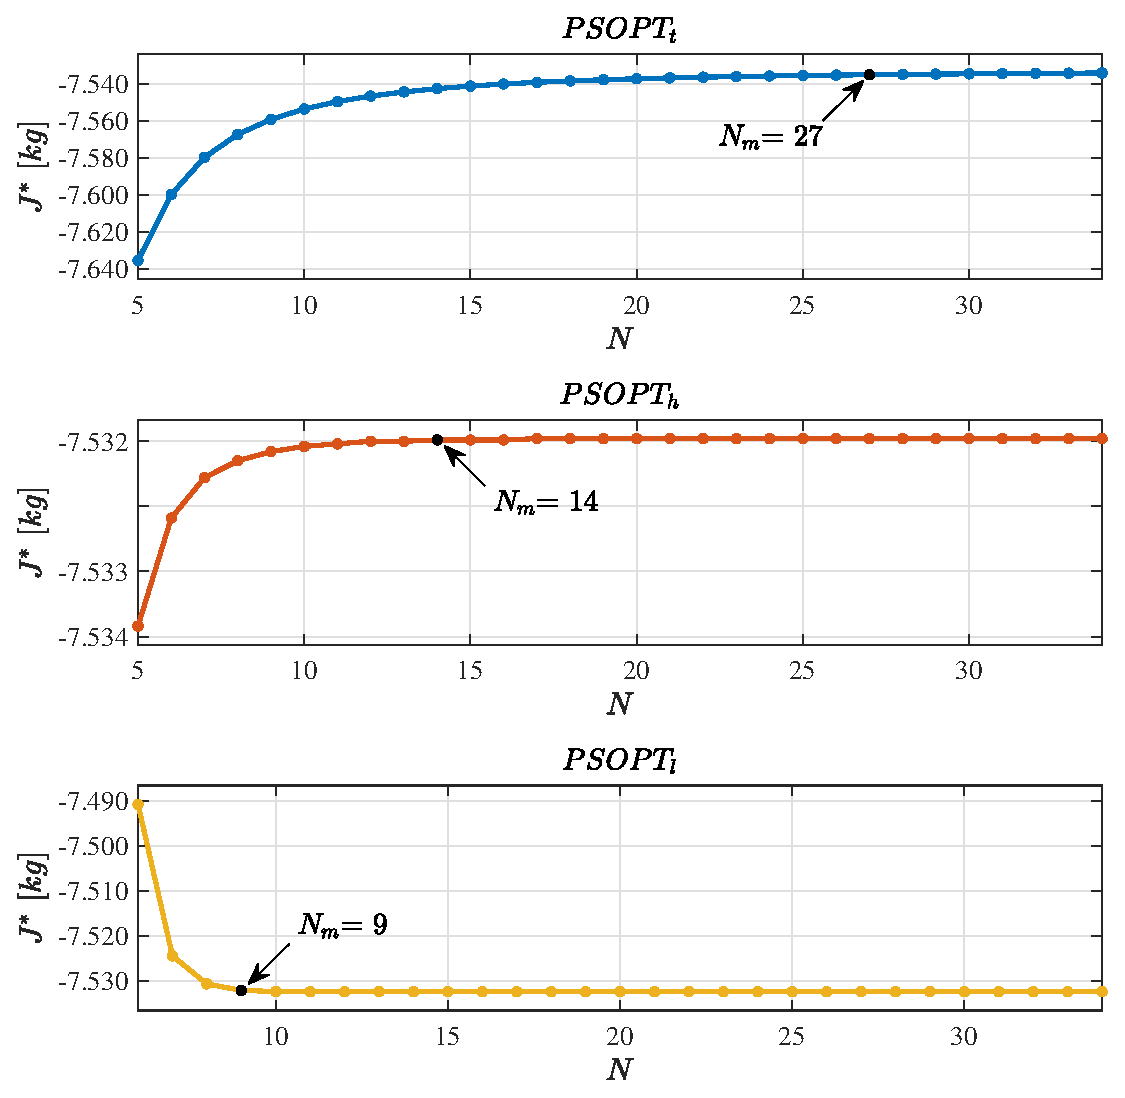
\includegraphics[width=0.7\linewidth]{fig/resultados/foguete/sens/J}
	\captionof{figure}[Influência do número de nós de colocação no valor da função objetivo para o problema do lançamento de um foguete]{Influência do número de nós de colocação $N$ no valor da função objetivo $J^*$ para o problema do lançamento de um foguete.}
	\label{fig:foguete:sensibilidade:J}
	\vspace{\onelineskip}
\end{minipage}

\todo[inline, color=pink, size=normalsize]{Análise da análise de sensibilidade $ J \times N $}

Diante dos resultados apresentados na Figura \ref{fig:foguete:sensibilidade:J}, vale ressaltar apenas que os $ J^* $ associados a todos os métodos convergiram com o aumento de $ N $, tendo os $ J^* $ relacionados ao $ PSOPT_t $ e ao $ PSOPT_h $ crescido com o aumento de $ N $, e aqueles atribuídos ao $ PSOPT_l $ diminuído com o crescimento de $ N $. Esse comportamento se deve às propriedades numéricas de cada tipo de colocação. 

\todo[inline, color=pink, size=normalsize]{Apresentação da tabela dos dados obtidos para $ N = N_m $}

Os resultados obtidos a partir da resolução do estudo de caso em análise são apresentados na Tabela \ref{tab:foguete:raw} e foram obtidos considerando-se $ N = N_m $. Adota-se $ J^* $ como o custo ótimo atribuído à solução obtida, $ t_p $ como o tempo de processamento médio, $ s_t $ como o desvio padrão atribuído a $ t_p $, $ n_{aval} $ como o número de avaliações da função objetivo, e $ \Delta c_{max} $ como a máxima violação das restrições. Ainda na Tabela \ref{tab:foguete:raw} são apresentadas as métricas referentes às análises de sensibilidade empregadas na avaliação dos pacotes utilizados. Mais especificamente, o número de execuções bem sucedidas $ N_s $, e a relação $ N_s\% $ entre $ N_s $ e o número total de execuções, nesse caso igual a 30.

\begin{table}
	\centering
	\caption[Métricas obtidas para o problema do foguete]{Métricas obtidas para o problema do lançamento de um foguete. Os melhores $ N_m $, $ J^* $, $ t_p $, $ n_{aval} $ e $ N_s\% $ se encontram destacados.}
	\label{tab:foguete:raw}
	\begin{tabular}{@{}ccccccccc@{}}
		\toprule
		Método       & $N_m$                             & $J^*$                                       & $t_p$ {[}$s${]}                         & $s_t$ {[}$s${]}                         & $n_{aval}$                          & $\Delta c_{max}$                         & $N_s$ & $N_s\%$                                  \\ \midrule
		$PSOPT_t$    & 27                                & {\color[HTML]{009901} \textbf{-7534,94000}} & 4,82663                                 & 0,14216                                 & {\color[HTML]{009901} \textbf{331}} & 1,35e-08                                 & 30    & {\color[HTML]{009901} \textbf{100,00\%}} \\
		$PSOPT_h$    & 14                                & -7532,49000                                 & 2,34095                                 & 0,12260 & 364                                 & 1,35e-08                                 & 30    & {\color[HTML]{009901} \textbf{100,00\%}} \\
		$PSOPT_l$    & {\color[HTML]{009901} \textbf{9}} & -7532,18000                                 & {\color[HTML]{009901} \textbf{1,88649}} & 0,14480                                 & 475                                 & 2,55e-10 & 29    & 96,67\%                                  \\
		$FALCON$     & -                                 & -                                           & -                                       & -                                       & -                                   & -                                        & -     & -                                        \\
		$COPILOTS_t$ & -                                 & -                                           & -                                       & -                                       & -                                   & -                                        & -     & -                                        \\
		$COPILOTS_h$ & -                                 & -                                           & -                                       & -                                       & -                                   & -                                        & -     & -                                        \\ \bottomrule
	\end{tabular}
\end{table}

\todo[inline, color=pink, size=normalsize]{Análise dos dados obtidos para $ N = N_m $}
 
Primeiramente, verifica-se que são atribuído ao $ PSOPT_l $ e ao $ PSOPT_t $ o menor e maior $ N_m $, respectivamente. Esses resultados justificam o baixo $ t_p $ associado ao $ PSOPT_l $ e o baixo $ J^* $ atribuído ao $ PSOPT_t $, e se devem às propriedades numéricas das colocações trapezoidal e pseudo-espectral, e aos tipos de interpolação associados a cada colocação. Ainda assim, é preciso ressaltar que, pelos mesmo motivos, é atribuído ao $ PSOPT_t $ o menor $ n_{aval} $.

Observa-se que com o aumento dos $ t_p $ associados a cada método, verifica-se a diminuição dos respectivos $ n_{aval} $. Esse resultado indica uma relação direta entre $ N_m $ e $ t_p $, de forma que $ t_p $ cresce com o aumento de $ N_m $. Em contrapartida, apesar de existir uma relação entre $ N_m $ e $ n_{aval} $, nota-se que $ n_{aval} $ é mais dependente do tipo de colocação empregado. De fato, os $ n_{aval} $ associados à colocação trapezoidal tendem a ser menores que os atribuídos à colocação Hermite-Simpson, que faz uso de nós de colocação intermediários para determinação dos controles.

Por fim, vale ressaltar que, empregando qualquer um dos métodos, é possível atingir um alto $ N_s\% $, igual ou consideravelmente próximo a 100\%. 
 
\todo[inline, color=pink, size=normalsize]{Apresentação das trajetórias de estados e controles}

As trajetórias de altitude $ h $, massa $ m $, e velocidade absoluta $ v $ obtidas considerando-se $ N = N_m $ são introduzidas nos gráficos das Figuras \ref{fig:foguete:x:h}, \ref{fig:foguete:x:m} e \ref{fig:foguete:x:v}. As trajetórias dos controles por sua vez são apresentadas nas Figuras \ref{fig:foguete:u:u_x}, \ref{fig:foguete:u:u_y} e \ref{fig:foguete:u:u_z}. Os pontos nesses gráficos representam os valores assumidos pela altitude, massa, velocidade absoluta, ou pelos controles em cada nó de colocação, enquanto as linhas contínuas representam as trajetórias interpoladas a partir desses pontos.

\noindent
\begin{minipage}{\textwidth}
	\vspace{\onelineskip}
	\centering
	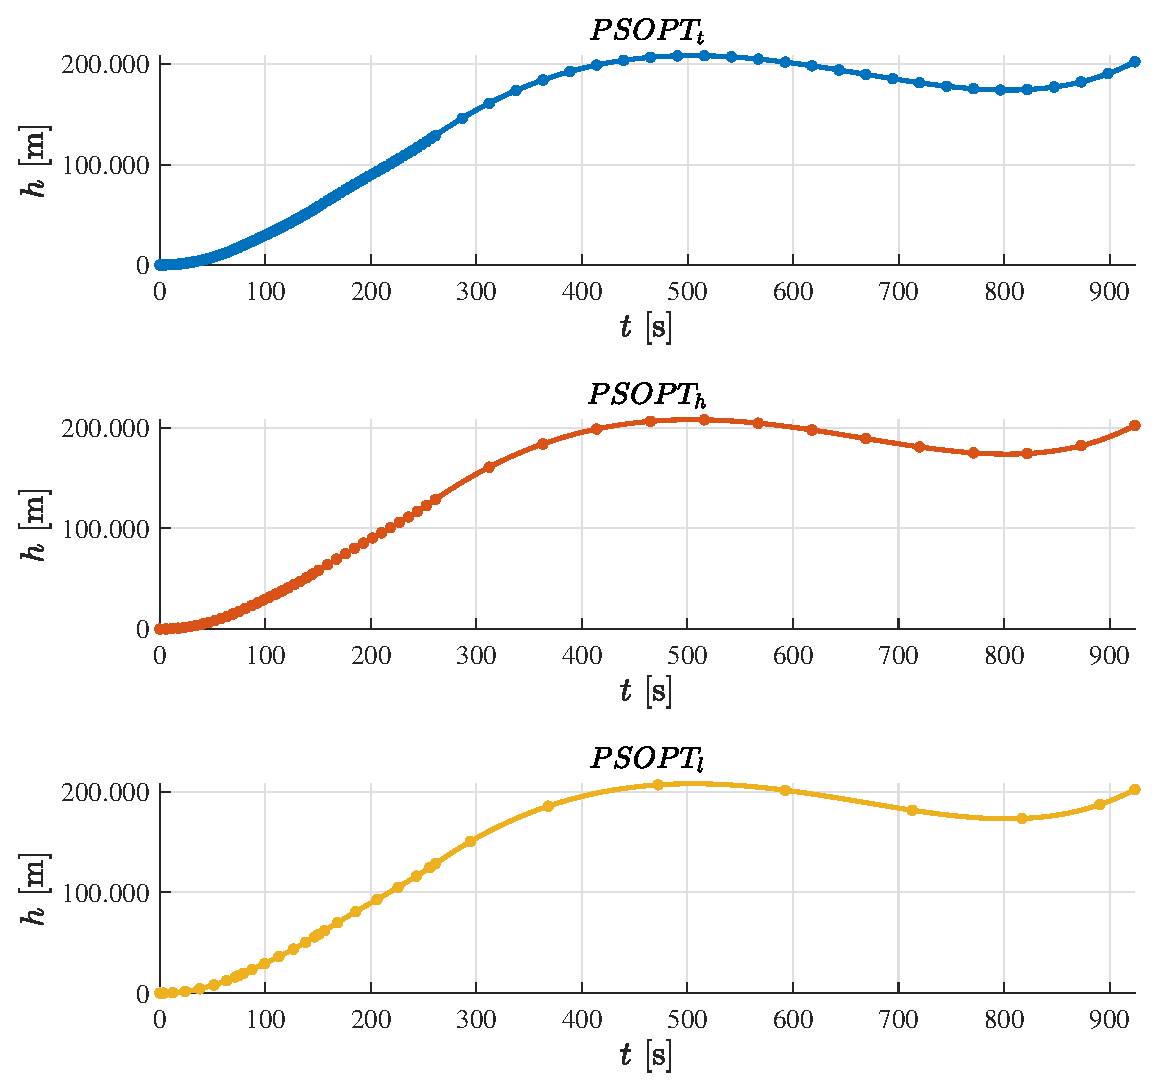
\includegraphics[width=0.7\linewidth]{fig/resultados/foguete/traj/x/h}
	\captionof{figure}[Variável $h(t)$ para o problema do lançamento de um foguete]{Variável $h(t)$ para o problema do lançamento de um foguete. Os pontos em cada um dos gráficos representam os valores discretizados, enquanto as linhas contínuas representam as trajetórias interpoladas.}
	\label{fig:foguete:x:h}
	\vspace{\onelineskip}
\end{minipage}

\noindent
\begin{minipage}{\textwidth}
	\vspace{\onelineskip}
	\centering
	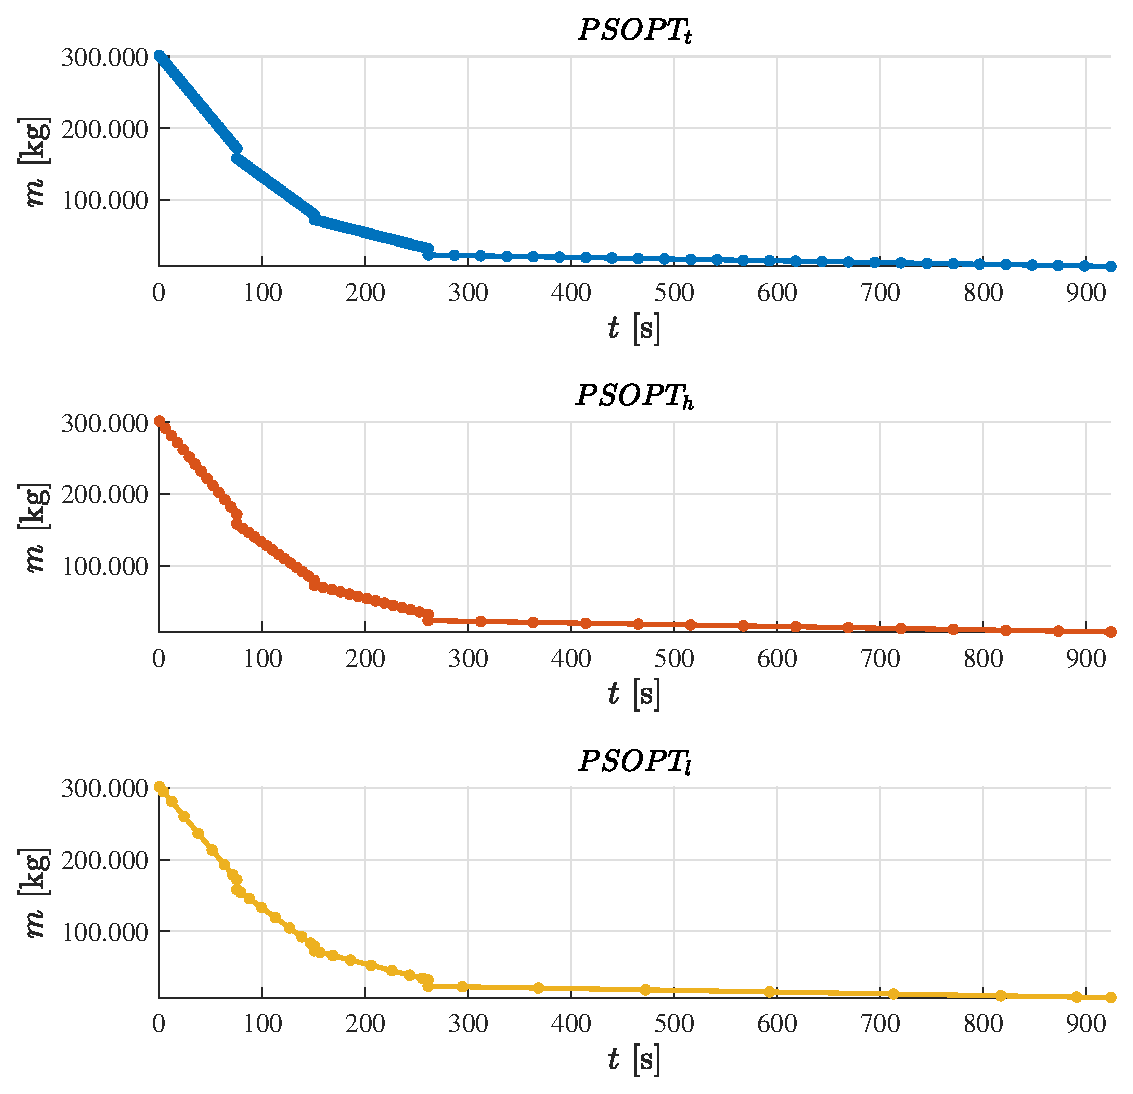
\includegraphics[width=0.7\linewidth]{fig/resultados/foguete/traj/x/m}
	\captionof{figure}[Variável $m(t)$ para o problema do lançamento de um foguete]{Variável $m(t)$ para o problema do lançamento de um foguete. Os pontos em cada um dos gráficos representam os valores discretizados, enquanto as linhas contínuas representam as trajetórias interpoladas.}
	\label{fig:foguete:x:m}
	\vspace{\onelineskip}
\end{minipage}

\noindent
\begin{minipage}{\textwidth}
	\vspace{\onelineskip}
	\centering
	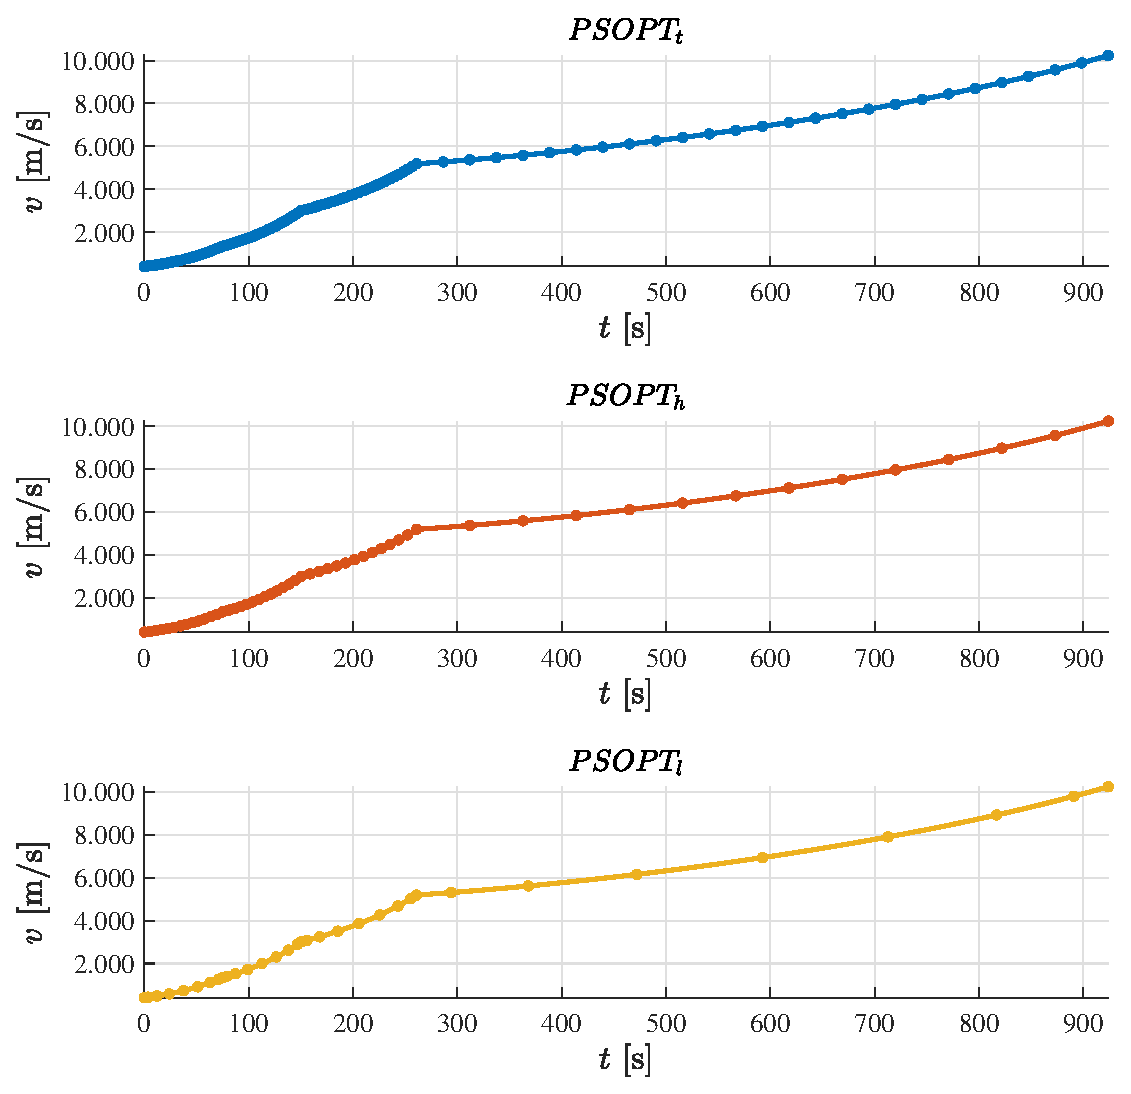
\includegraphics[width=0.7\linewidth]{fig/resultados/foguete/traj/x/v}
	\captionof{figure}[Variável $v(t)$ para o problema do lançamento de um foguete]{Variável $v(t)$ para o problema do lançamento de um foguete. Os pontos em cada um dos gráficos representam os valores discretizados, enquanto as linhas contínuas representam as trajetórias interpoladas.}
	\label{fig:foguete:x:v}
	\vspace{\onelineskip}
\end{minipage}

\noindent
\begin{minipage}{\textwidth}
	\vspace{\onelineskip}
	\centering
	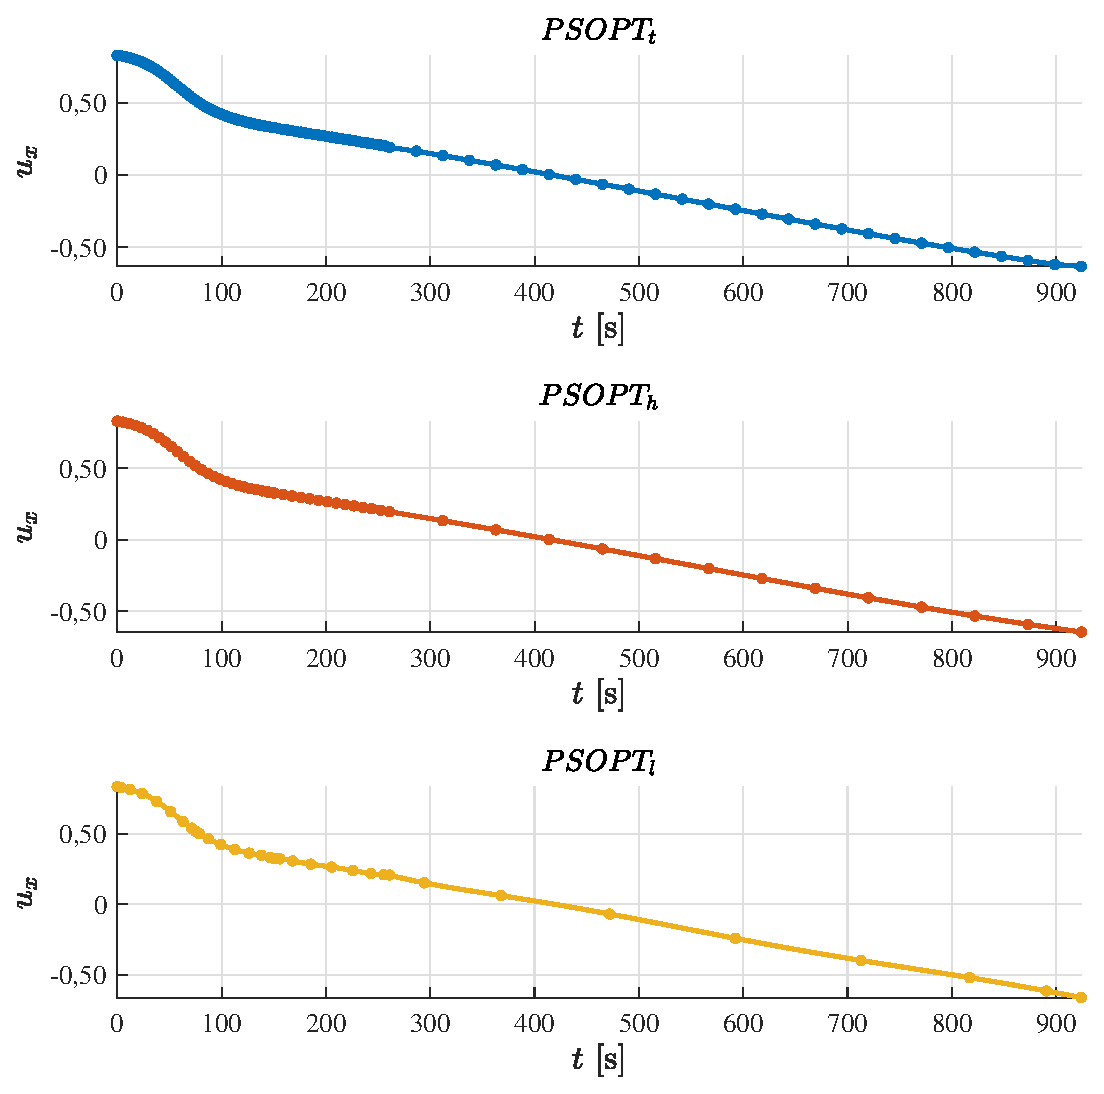
\includegraphics[width=0.7\linewidth]{fig/resultados/foguete/traj/u/u1}
	\captionof{figure}[Variável de controle $u_x(t)$ para o problema do lançamento de um foguete]{Variável de controle $u_x(t)$ para o problema do lançamento de um foguete. Os pontos em cada um dos gráficos representam os valores discretizados, enquanto as linhas contínuas representam as trajetórias interpoladas.}
	\label{fig:foguete:u:u_x}
	\vspace{\onelineskip}
\end{minipage}

\noindent
\begin{minipage}{\textwidth}
	\vspace{\onelineskip}
	\centering
	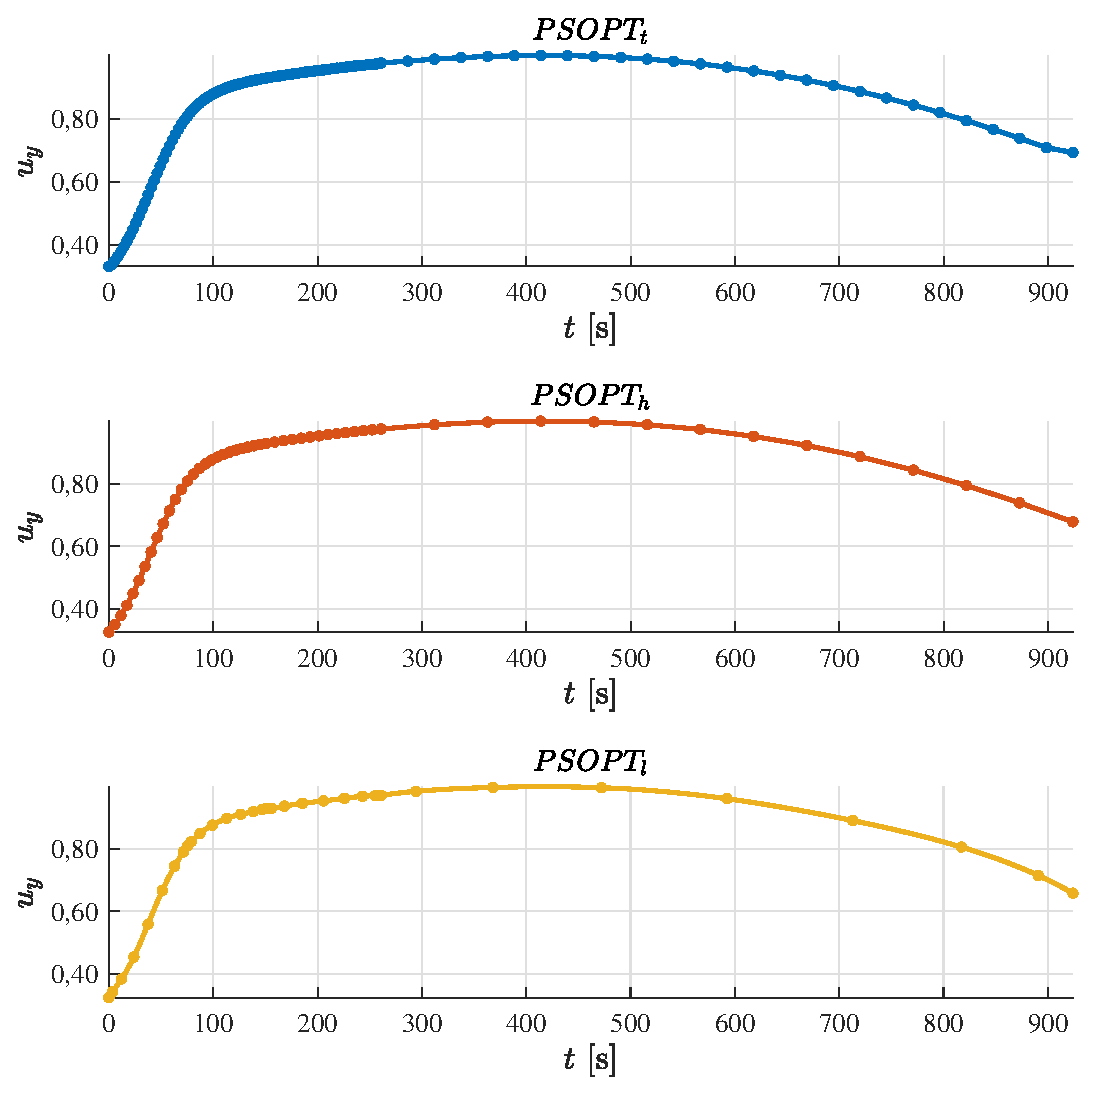
\includegraphics[width=0.7\linewidth]{fig/resultados/foguete/traj/u/u2}
	\captionof{figure}[Variável de controle $u_y(t)$ para o problema do lançamento de um foguete]{Variável de controle $u_y(t)$ para o problema do lançamento de um foguete. Os pontos em cada um dos gráficos representam os valores discretizados, enquanto as linhas contínuas representam as trajetórias interpoladas.}
	\label{fig:foguete:u:u_y}
	\vspace{\onelineskip}
\end{minipage}

\noindent
\begin{minipage}{\textwidth}
	\vspace{\onelineskip}
	\centering
	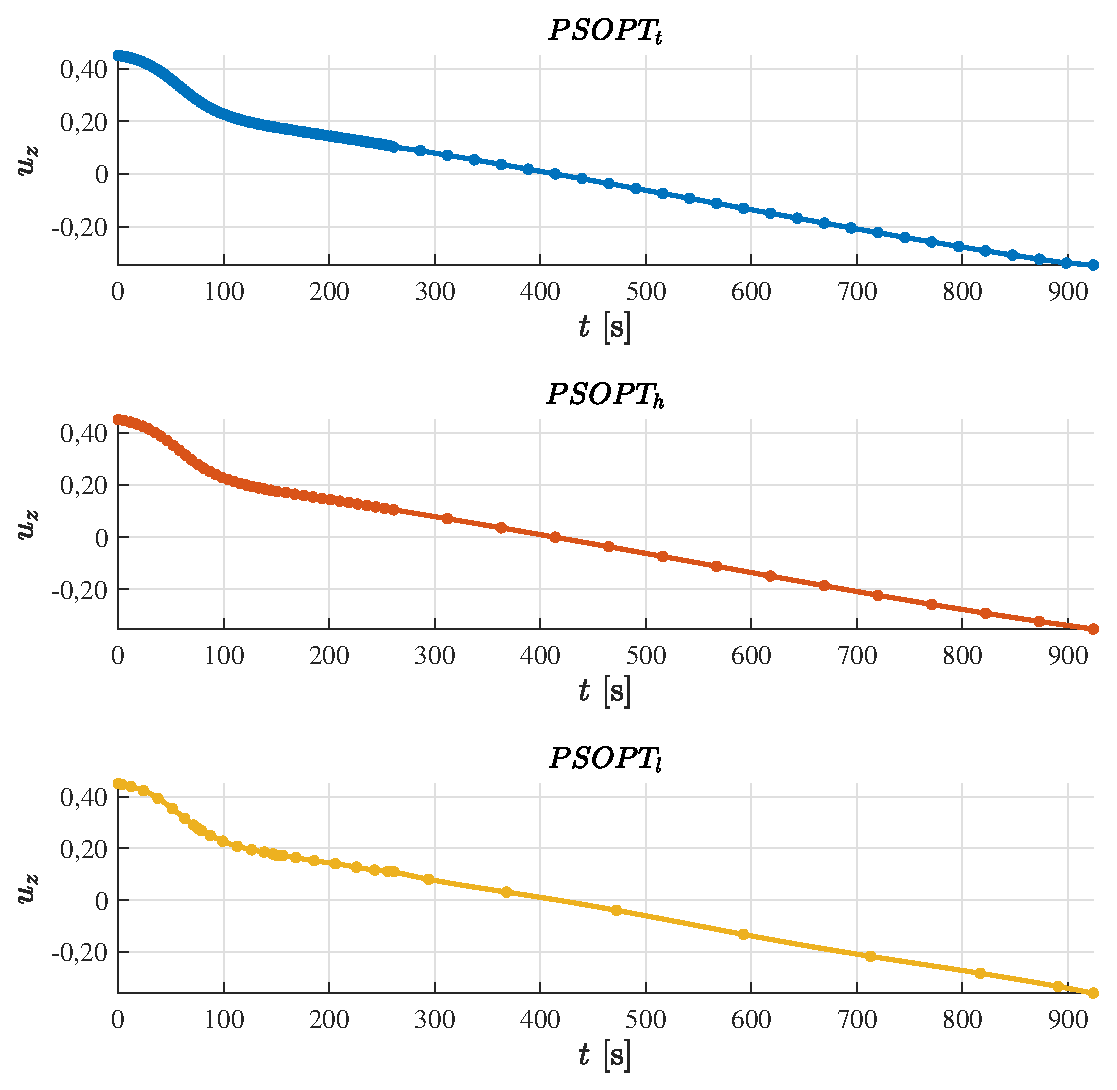
\includegraphics[width=0.7\linewidth]{fig/resultados/foguete/traj/u/u3}
	\captionof{figure}[Variável de controle $u_z(t)$ para o problema do lançamento de um foguete]{Variável de controle $u_z(t)$ para o problema do lançamento de um foguete. Os pontos em cada um dos gráficos representam os valores discretizados, enquanto as linhas contínuas representam as trajetórias interpoladas.}
	\label{fig:foguete:u:u_z}
	\vspace{\onelineskip}
\end{minipage}

\todo[inline, color=pink, size=normalsize]{Análise das trajetórias de estados e controles}

Primeiramente, observa-se que as trajetórias de altitude e velocidade absoluta, diretamente relacionadas a $ \mathbf{r}(t) $ e $ \mathbf{v}(t) $, são de fato contínuas, o que indica o atendimento das restrições \eqref{eq:foguete:rContinua} e \eqref{eq:foguete:vContinua}. Em contrapartida, são claras as descontinuidades presentes nas trajetórias de massa, ocasionadas pelo descarte de propulsores ou estágios cujo combustível já tenha sido queimado. Tais descontinuidades ocorrem em $ t = 75,2 $ s, $ t = 150,4 $ s, e $ t = 261 $ s. 

Além disso, cabe ressaltar que as trajetórias de altitude, velocidade, massa e controle, obtidas pelo emprego de cada um dos métodos avaliados são muito semelhantes umas às outras.  

\todo[inline, color=pink, size=normalsize]{Apresentação dos gráficos de trajetória complexos caso haja}

No gráfico da Figura \ref{fig:foguete:avancado} está representada a trajetória percorrida pelo foguete. Nesse caso foi empregado o sistema de coordenadas introduzido na Figura \ref{fig:foguete:latitudeLongitude}, de forma que a posição do foguete é determinada com base na latitude e na longitude. A construção do gráfico em questão baseia-se nos resultados obtidos por meio do $ PSOPT_t $, pacote ao qual associa-se o menor $ J^* $. Os pontos no gráfico advém dos valores assumidos por $ \mathbf{r}(t) $ e $ \mathbf{v}(t) $ nos nós de colocação, enquanto a linha continua que conecta esses pontos representa a trajetória computada com base nas trajetórias obtidas por meio da interpolação desses valores. Vale ressaltar que o método no qual se baseia essa interpolação depende do tipo de colocação empregado. 

Uma vez que o sistema de coordenadas baseado na latitude e na longitude se move juntamente com a Terra, é necessário que uma data e um horário sejam especificados para que a conversão $ \big( \mathbf{r}(t), \mathbf{v}(t) \big) \rightarrow \big( \text{latitude}, \text{longitude} \big)$ seja realizada. Nesse caso adota-se que o foguete é lançado no dia 26 de agosto de 1998 (data do primeiro lançamento de um Delta III) às 7:05 AM. A conversão a partir da qual foi determinada a trajetória apresentada na Figura \ref{fig:foguete:avancado} foi realizada no Matlab\textsuperscript{\textregistered} por meio da função \texttt{eci2lla()}. 

\noindent
\begin{minipage}{\textwidth}
	\vspace{\onelineskip}
	\centering
	\includegraphics[width=1\linewidth]{fig/resultados/foguete/obs/adv}
	\captionof{figure}[Trajetória percorrida pelo Delta III]{Trajetória percorrida pelo Delta III.}
	\label{fig:foguete:avancado}
	\vspace{\onelineskip}
\end{minipage}

\todo[inline, color=pink, size=normalsize]{Apresentação das análises de sensibilidade $ N \times t_p $ e $ N \times n_{aval} $}

Foi também verificado o impacto que o aumento no número de nós de colocação tem no tempo de processamento, Figura \ref{fig:foguete:sensibilidade:t}, e no número de avaliações da função objetivo, Figura \ref{fig:foguete:sensibilidade:naval}. Acima de cada um dos gráficos introduzidos nessas figuras, são apresentados $ \Delta t_p = max\{t_p\} - min\{t_p\} $ e $ \Delta n_{aval} = max\{n_{aval}\} - min\{n_{aval}\} $. Os pontos nesses gráficos representam os valores atribuídos a $ t_p $ ou a $ n_{aval} $ para cada um dos $ N $ considerados, enquanto as linhas contínuas representam curvas de tendência, obtidas por meio de regressões lineares. O coeficiente de determinação $ R^2 $ associado a cada regressão é indicado nos gráficos. Os valores de $ N $ empregados na geração desses dados são iguais àqueles considerados na verificação da relação entre $ J^* $ e $ N $. 

\noindent
\begin{minipage}{\textwidth}
	\vspace{\onelineskip}
	\centering
	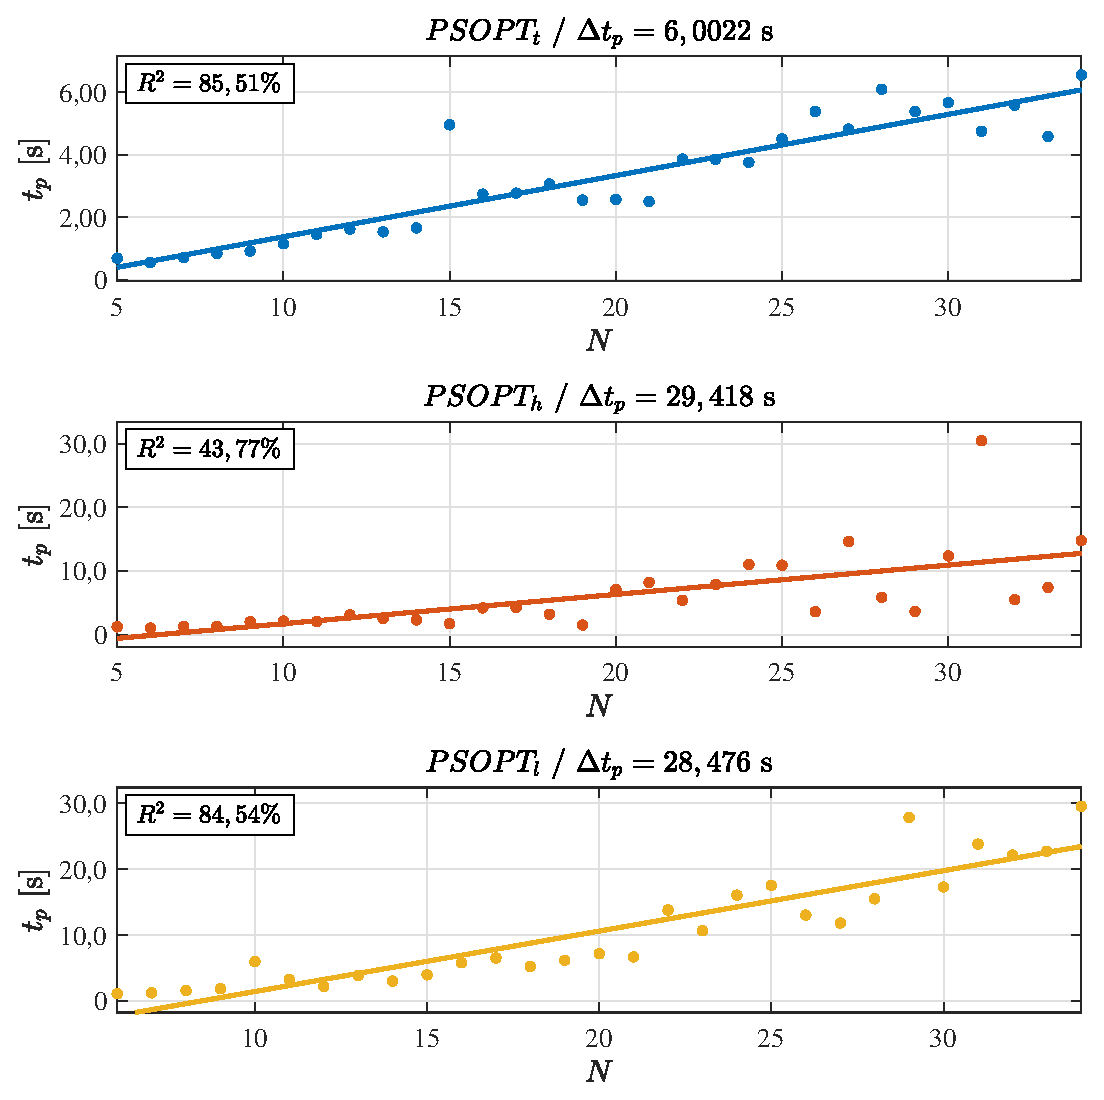
\includegraphics[width=0.7\linewidth]{fig/resultados/foguete/sens/t}
	\captionof{figure}[Relação entre o tempo de processamento e o número de nós de colocação para o problema do lançamento de um foguete]{Relação entre o tempo de processamento $ t_p $ e o número de nós de colocação $ N $ para o problema do lançamento de um foguete.}
	\vspace{\onelineskip}
\end{minipage}

\noindent
\begin{minipage}{\textwidth}
	\vspace{\onelineskip}
	\centering
	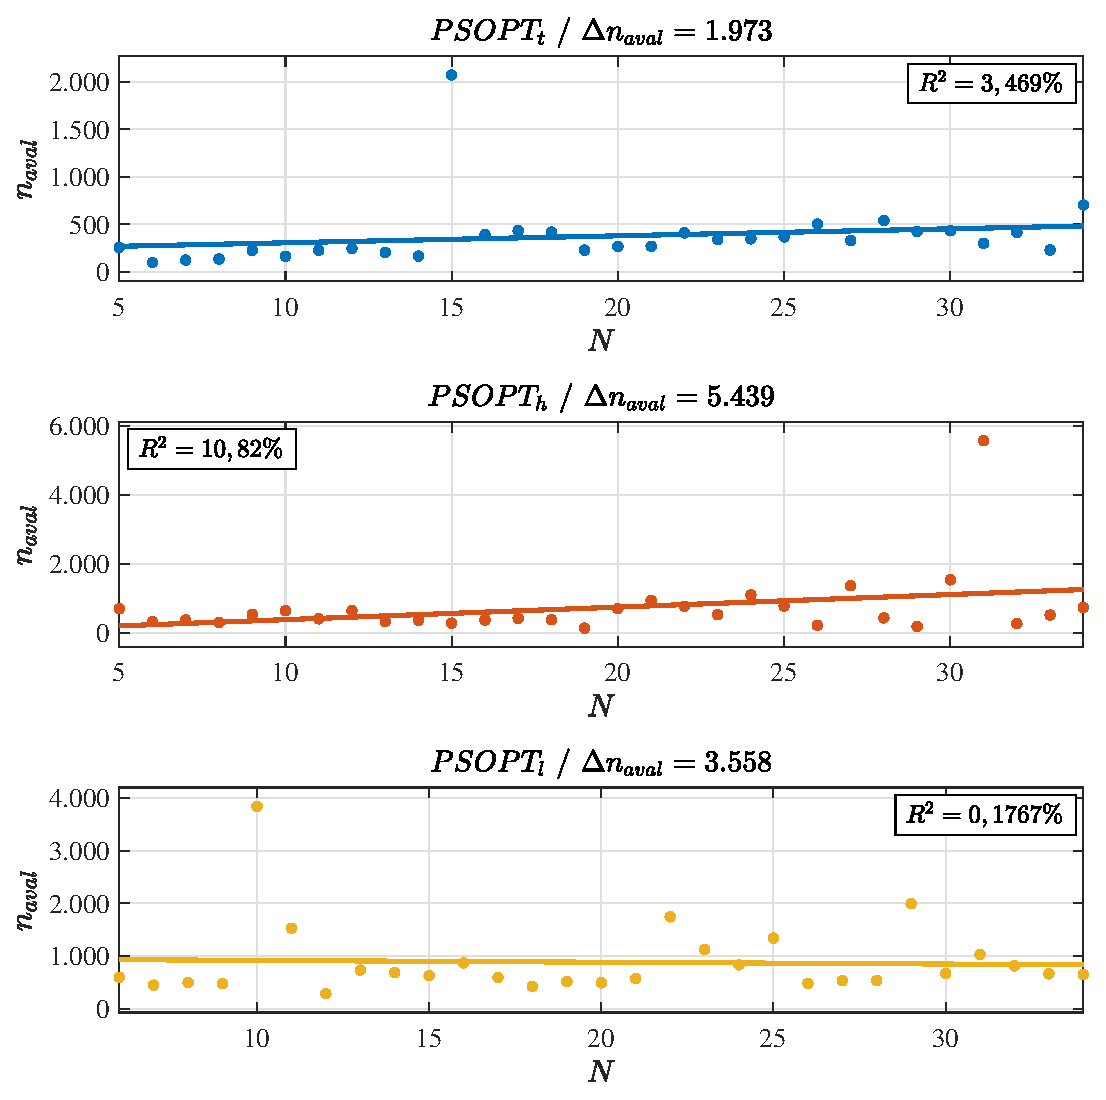
\includegraphics[width=0.7\linewidth]{fig/resultados/foguete/sens/eval}
	\captionof{figure}[Relação entre o número de avaliações da função objetivo e o número de nós de colocação para o problema do lançamento de um foguete]{Relação entre o número de avaliações da função objetivo $ n_{aval} $ e o número de nós de colocação $ N $ para o problema do lançamento de um foguete.}
	\label{fig:foguete:sensibilidade:naval}
	\vspace{\onelineskip}
\end{minipage}

\todo[inline, color=pink, size=normalsize]{Análise das análises de sensibilidade $ N \times t_p $ e $ N \times n_{aval} $}

Primeiramente, verifica-se que os $ t_p $ e $ n_{aval} $ associados ao $ PSOPT_t $ foram menos sensíveis ao aumento de $ N $ que os atribuídos aos demais métodos, dados os $ \Delta t_p $ e $ \Delta n_{aval} $ associados a cada método. Esse resultado se deve às propriedades numéricas da colocação trapezoidal. 

Verifica-se uma relação quase linear entre $ N $ e os $ t_p $ associados ao $ PSOPT_t $ e ao $ PSOPT_l $, dados os respectivos $ R^2 $, bem próximos de 100\%. No caso do $ PSOPT_h $, não é possível verificar tal relação, uma vez que o $ t_p $ associado a esse método apresenta picos para $ N > 25 $. 

Não é possível estabelecer uma relação linear entre $ N $ e os $ n_{aval} $ associados a nenhum dos métodos, dados os respectivos $ R^2 $, que são consideravelmente baixos. A dificuldade em estabelecer uma relação linear entre $ N $ e $ n_{aval} $ nesse caso se deve ao aparecimento de picos em $ n_{aval} $ que provavelmente estão relacionados ao método empregado na inicialização dos estados e controles. Vale ressaltar que a posição e velocidade finais $ \mathbf{r_f} $ e $ \mathbf{v_f} $, empregadas na inicialização dos estados das últimas duas fases, foram obtidas considerando-se $ \nu = 0 $. No entanto, essa não é a anomalia verdadeira atribuída à solução obtida. Além disso, é possível que assumir um palpite inicial em que os estados e controles se mantenham constantes ao longo de toda a fase não seja a melhor abordagem. 

Nota-se que o $ n_{aval} $ associado ao $ PSOPT_h $ é mais sensível ao aumento de $ N $ que os atribuídos aos demais métodos, o que pode ser verificado pela análise de $ \Delta n_{aval} $. Esse comportamento se deve às propriedades numéricas associadas à colocação Hermite-Simpson, que depende do estabelecimento de nós de colocação intermediários para a determinação dos controles, o que aumenta consideravelmente o número de variáveis de projeto associado ao PPNL. 

Por fim, destaca-se que, como esperado, picos em $ n_{aval} $ ocasionam picos em $ t_p $. Tal relação entre os picos de $ n_{aval} $ e $ t_p $ pode ser verificada em $ N = 15 $, no caso do $ PSOPT_t $, em $ N = 31 $ no caso do $ PSOPT_h $, e em $ N = 29 $ no caso do $ PSOPT_l $. De fato, uma vez que leva-se um determinado tempo para que a avaliação da função objetivo seja realizada, o aumento de $ n_{aval} $ é um dos fatores associados ao crescimento de $ t_p $. 

\todo[inline, color=pink, size=normalsize]{Observações adicionais sobre os resultados obtidos no estudo de caso - Conversão de posição e velocidade pra coordenadas orbitais e aproximações utilizadas nesse caso}

\subsection{Computação dos elementos orbitais}

Como enunciado anteriormente, a órbita a ser atingida pelo Delta III é definida a partir dos elementos orbitais $ a(t) $, $ e(t) $, $ i(t) $, $ \Omega(t) $, e $ \omega(t) $, que devem ser computados a partir de $ \mathbf{r}(t) $ e $ \mathbf{v}(t) $. Para tanto, obtém-se primeiramente $ a(t) $ empregando-se \eqref{eq:foguete:aOrbital}.
%
\begin{equation}
	\label{eq:foguete:aOrbital}
	a(t) = \frac{1}{ \cfrac{2}{|\mathbf{r}(t)|} - \cfrac{|\mathbf{v}(t)|^2}{\mu}} 
\end{equation}

Em seguida, definem-se $ {\bm \eta}(t) $ e $ \mathbf{e'}(t) $
%
\begin{equation}
	\begin{gathered}
		{\bm \eta}(t) = \begin{bmatrix} \eta_x(t) & \eta_y(t) & \eta_z(t) \end{bmatrix}^T  = \mathbf{r}(t) \times \mathbf{v}(t) \\
		\mathbf{e'}(t) = \begin{bmatrix} e'_x(t) & e'_y(t) & e'_z(t) \end{bmatrix}^T = \frac{\mathbf{v}(t) \times {\bm \eta}(t)}{\mu} - \frac{\mathbf{r}(t)}{|\mathbf{r}(t)|}
	\end{gathered}
\end{equation}
%
de forma que $ e(t) $ e $ i(t) $ sejam determinados pelo emprego de \eqref{eq:foguete:eiOrbital}.
%
\begin{equation}
	\label{eq:foguete:eiOrbital}
	\begin{gathered}
		e(t) = |\mathbf{e'}(t)| \\
		i(t) = cos^{-1} \frac{\eta_z(t)}{|{\bm \eta}(t)|} 
	\end{gathered}
\end{equation}

Por fim, partindo-se da definição de $ \mathbf{n}(t) $
%
\begin{equation}
	\mathbf{n}(t) = \begin{bmatrix} n_x(t) & n_y(t) & n_z \end{bmatrix}^T = \begin{bmatrix} -\eta_y(t) & \eta_x(t) & 0 \end{bmatrix}^T 
\end{equation}
%
determinam-se $ \Omega(t) $ e $ \omega(t) $ de acordo com \eqref{eq:foguete:wOmegaOrbital} \cite{schwarz_cartesian_2017}.
%
\begin{equation}
	\label{eq:foguete:wOmegaOrbital}
	\begin{gathered}
		\Omega(t) = \begin{cases}
		cos^{-1} \cfrac{n_x(t)}{|\mathbf{n}(t)|} &\text{ se } n_y(t) \geq 0 \\
		2 \pi - cos^{-1} \cfrac{n_x(t)}{|\mathbf{n}(t)|} &\text{ se } n_y(t) < 0
		\end{cases} \\
		\omega(t) = \begin{cases}
		cos^{-1} \cfrac{\mathbf{n}(t) \bigcdot \mathbf{e'}(t)}{|\mathbf{n}(t)||\mathbf{e'}(t)|} &\text{ se } e'_z(t) \geq 0 \\
		2 \pi - cos^{-1} \cfrac{\mathbf{n}(t) \bigcdot \mathbf{e'}(t)}{|\mathbf{n}(t)||\mathbf{e'}(t)|} &\text{ se } e'_z(t) < 0
		\end{cases}
	\end{gathered}
\end{equation}

Ressalta-se que as descontinuidades associadas às definições de $ \Omega(t) $ e $ \omega(t) $ podem impossibilitar a resolução do estudo de caso em análise. Para resolver esse problema, reescreve-se \eqref{eq:foguete:wOmegaOrbital} da seguinte forma:
%
\begin{equation}
	\begin{gathered}
		\Omega(t) = U_s\big( n_y(t) \big) \, cos^{-1} \frac{n_x(t)}{|\mathbf{n}(t)|} + U_s\big( -n_y(t) \big) \left( 2 \pi - cos^{-1} \frac{n_x(t)}{|\mathbf{n}(t)|} \right) \\ 
		\omega(t) = U_s\big( e'_z(t) \big) \, cos^{-1} \cfrac{\mathbf{n}(t) \bigcdot \mathbf{e'}(t)}{|\mathbf{n}(t)||\mathbf{e'}(t)|} + U_s\big( -e'_z(t) \big) \left( 2 \pi - cos^{-1} \cfrac{\mathbf{n}(t) \bigcdot \mathbf{e'}(t)}{|\mathbf{n}(t)||\mathbf{e'}(t)|} \right) \\ 
	\end{gathered}
\end{equation}
%
sendo $ U_s(x) $ a função degrau. Em seguida, tratam-se as descontinuidades associadas a \eqref{eq:foguete:wOmegaOrbital} substituindo-se $ U_s(x) $ por uma aproximação suave $ U_s'(x) $, Figura \ref{fig:foguete:aproximacaoDegrau} \cite{becerra_psopt_2019}. Nesse caso adota-se
%
\begin{equation}
	\label{eq:foguete:apxDegrau}
	U_s'(x) = 0,5 \left( 1 + tanh \left( \frac{x}{0,1} \right) \right)
\end{equation}
%
tendo sido o parâmetro $ 0,1 $, que divide $ x $, escolhido por meio de um processo de experimentação numérica. 

\noindent	
\begin{minipage}{\textwidth}
	\vspace{\onelineskip}
	\centering
	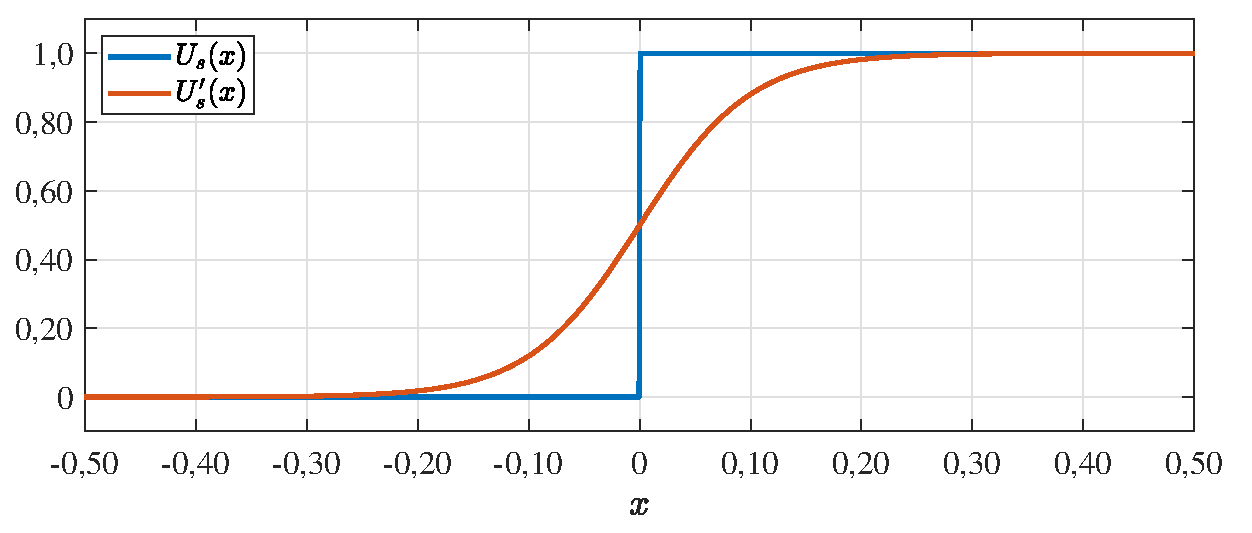
\includegraphics[width=1\linewidth]{fig/resultados/foguete/obs/apxDegrau}
	\captionof{figure}[Representação da aproximação utilizada na suavização da função degrau]{Comparação entre a função degrau $ U_s(x) $ e a aproximação suave $ U_s'(x) $, introduzida em \eqref{eq:foguete:apxDegrau}.}
	\label{fig:foguete:aproximacaoDegrau}
	\vspace{\onelineskip}
\end{minipage}
